\documentclass{article}

\PassOptionsToPackage{authoryear,round}{natbib}
\usepackage{neurips_2026}

\usepackage[utf8]{inputenc}
\usepackage[T1]{fontenc}
\usepackage{amsmath,amssymb,amsthm,mathtools}
\usepackage{amsfonts}
\usepackage{bbm}
\usepackage{booktabs}
\usepackage{enumitem}
\usepackage{graphicx}
\usepackage{xcolor}
\usepackage[colorlinks=true,linkcolor=blue,citecolor=blue,urlcolor=blue]{hyperref}
\usepackage[nameinlink,noabbrev]{cleveref}

\title{Empirical Reproduction of Prediction-Powered Inference With Calibration Baselines}
\author{Lars van der Laan}

\begin{document}

\maketitle

\section{Empirical Illustration}
\label{sec:empirical}
We evaluate the proposed calibration-based estimators on the mean-estimation benchmarks from the original PPI ecosystem \citep{ppi2023,angelopoulos2023ppi}. The aim is not to replace the original comparison, but to test when one-dimensional recalibration of the prediction score improves semisupervised mean inference. We use the official \texttt{ppi\_py} datasets and preserve the labeled-sample-size grids from the original examples. For each labeled sample size \(n\), we repeatedly split the fully labeled benchmark into a labeled subset of size \(n\) and an unlabeled subset of size \(N\), run all estimators on the same split, and treat the full-sample mean as ground truth. The reported results average over 5000 random splits per \(n\), which makes the coverage and interval-width trends materially smoother while still keeping the benchmark tractable.

\paragraph{Benchmarks and baselines.}
We study the \texttt{forest}, \texttt{galaxies}, and semisupervised \texttt{census\_income} mean-estimation examples from the official benchmark suite. The retained baselines are the original labeled-only interval, the imputation benchmark on the binary-outcome datasets, the semisupervised linear regression baseline from \texttt{ppi\_py} that uses the full covariate vector, vanilla PPI, and the classical AIPW estimator built from the same prediction score. Here AIPW averages the score over the pooled covariate sample and keeps the usual labeled residual correction, so it is the natural semiparametric efficiency benchmark against which PPI should be compared. We then add three recalibration comparators that fit naturally into our framework: linear recalibration, Platt scaling on the binary-outcome datasets, and isotonic recalibration with a fixed minimum of 10 observations per bin. For the binary-outcome datasets we also report a Venn--Abers shrinkage variant. We do not include PPI+ or prognostic-score adjustment as separate baselines, since in the present one-score setting they are numerically equivalent to linear recalibration.

\paragraph{Metrics and main message.}
For each estimator we summarize Monte Carlo bias, empirical variance, MSE, Wald-interval coverage, and relative efficiency versus PPI, computed from empirical Monte Carlo variance. Estimated standard errors are used only internally to construct the Wald intervals; all displayed variability summaries in the paper are empirical Monte Carlo quantities. The results support a simple practical picture. First, AIPW is the natural pooled plug-in benchmark against which vanilla PPI should be compared. In finite samples the empirical variance ordering is not uniform across every dataset and sample size, but AIPW is often slightly more efficient on the balanced synthetic regimes and on the \texttt{forest} and \texttt{galaxies} benchmarks. Second, when the unlabeled sample is much larger than the labeled sample, AIPW and PPI become nearly indistinguishable, since the labeled contribution to the pooled plug-in term is then negligible. Third, recalibration can improve semisupervised inference when the score is genuinely miscalibrated, especially once the labeled sample is large enough for the second-stage calibrator to be learned stably. In that regime, linear recalibration often captures most of the available gain when the misspecification is mild, while monotone nonlinear calibration is more useful when the distortion is genuinely nonlinear.

This pattern appears clearly across the three reproduced benchmarks. In \texttt{forest}, where the original score is already strong, AIPW, PPI, and the calibration-based estimators are all very close, with only small MSE and interval-width differences, though AIPW typically has slightly smaller empirical variance than PPI. In \texttt{galaxies}, AIPW and PPI are again nearly tied, linear recalibration is the closest practical competitor, and the fixed-bin isotonic rule remains competitive without clearly dominating. In the more difficult \texttt{census\_income} benchmark, PPI and AIPW again track each other closely because the unlabeled sample is enormous relative to the labeled sample, while linear recalibration performs best on average over the full labeled-sample grid and the fixed-bin isotonic rule becomes competitive once enough labeled data are available. Thus the empirical story is consistent with the theory: calibration helps when the score is miscalibrated and the correction can be learned stably, while offering little benefit when the original score is already well behaved.

\begin{table}[t]
\centering
\small
\begin{tabular}{p{0.16\textwidth}p{0.34\textwidth}p{0.34\textwidth}}
\toprule
Dataset & Smaller labeled-sample regime & Larger labeled-sample regime \\
\midrule
\texttt{forest} & AIPW already weakly dominates vanilla PPI, so there is little reason to use PPI when the original score is already strong. & AIPW is clearly preferable to PPI, while additional recalibration changes little beyond modest MSE gains. \\
\texttt{galaxies} & AIPW and PPI are very close, but PPI offers no practical advantage over AIPW; LinearCal is the nearest recalibration competitor. & The leading score-based methods become nearly indistinguishable, so a simple linear correction is usually enough and vanilla PPI is not preferred to AIPW. \\
\texttt{census\_income} & PPI and AIPW are effectively indistinguishable because the unlabeled sample is enormous; flexible calibration can be too aggressive when the labeled sample is very small. & LinearCal is best on average, with IsoCal (min bin 10) also competitive once enough labeled data are available; PPI remains essentially tied with AIPW rather than better. \\
\bottomrule
\end{tabular}
\caption{Compact regime summary of the reproduced PPI benchmarks. The main empirical distinction is between small labeled-sample regimes, where simple or no recalibration is safer, and larger labeled-sample regimes, where recalibration can help when the score is miscalibrated.}
\label{tab:ppi-takeaways}
\end{table}

\begin{figure}[t]
\centering
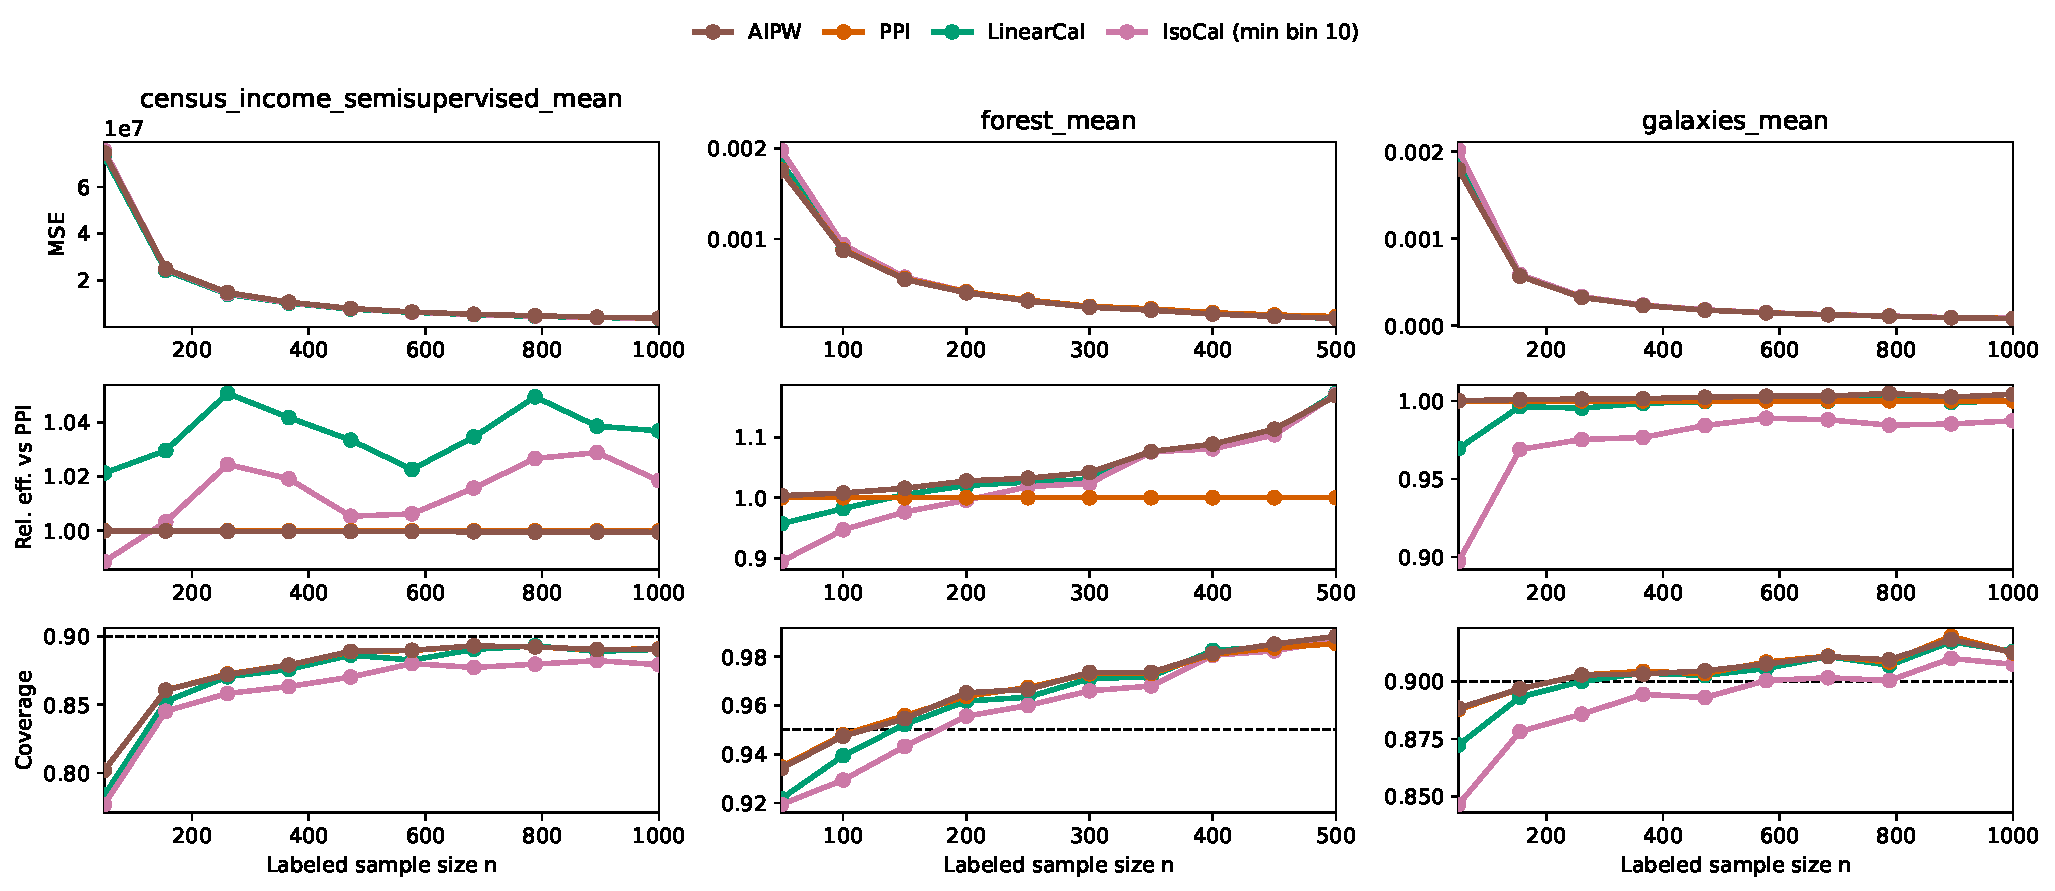
\includegraphics[width=\textwidth]{paper_assets/fig_paper_main_grid.pdf}
\caption{Main-text benchmark summary showing MSE, relative efficiency versus PPI, and coverage across the reproduced PPI benchmarks, restricted to the most informative score-based comparators: AIPW, PPI, LinearCal, and IsoCal (min bin 10). Relative efficiency is computed from empirical Monte Carlo variance, so values above one indicate improvement over vanilla PPI. The dashed horizontal line in the coverage panels marks the nominal target coverage, which is \(0.95\) for \texttt{forest} and \(0.90\) for \texttt{galaxies} and \texttt{census\_income}.}
\label{fig:ppi-main}
\end{figure}

\paragraph{Practical differences between recalibrators.}
The fixed-bin isotonic rule with a minimum of 10 observations per bin is the cheapest nonlinear calibrator and performs competitively once the labeled sample is moderately large, especially in \texttt{census\_income} and at some labeled sample sizes in \texttt{galaxies}. Platt scaling is numerically stable on the binary tasks and is a natural logistic alternative when over- or under-confidence is plausibly sigmoidal, but in these data it does not systematically outperform AIPW, linear recalibration, or the fixed-bin isotonic rule. Venn--Abers shrinkage can slightly tighten intervals on the binary tasks, but its MSE gains over simpler recalibrators are small and inconsistent. Taken together, the experiments suggest a simple practical hierarchy: prefer AIPW over vanilla PPI as the baseline score-based estimator; use linear recalibration when misspecification appears mild or the labeled sample is small; use the cheap isotonic rule when nonlinear correction is desired at low cost; and reserve Platt scaling or Venn--Abers mainly for binary-outcome robustness checks when sigmoidal shape or extra shrinkage is substantively motivated.

\appendix

\section{Additional empirical details}
\label{app:empirical}
This appendix records the benchmark construction used in \cref{sec:empirical}. We use the official \texttt{ppi\_py} real-data mean-estimation examples and preserve their labeled-sample-size grids. The \texttt{forest} experiment uses \(n \in \{50,100,\dots,500\}\), while \texttt{galaxies} and semisupervised \texttt{census\_income} use \(n \in \{50,155,261,366,472,577,683,788,894,1000\}\). For each \(n\), the remaining observations form the unlabeled sample. We rerandomize this split 5000 times at each \(n\), always evaluating all estimators on the same split and taking the full-sample mean as the benchmark truth.

The estimator set mirrors the original PPI comparison wherever possible. We report the labeled-only estimator, the imputation benchmark on binary-outcome tasks, the official semisupervised linear baseline from \texttt{ppi\_py}, vanilla PPI computed using the official \texttt{ppi\_py} implementation, and the classical AIPW estimator based on the same prediction score. We then add four calibration-based plug-in estimators: affine linear recalibration; Platt scaling on the binary-outcome benchmarks; isotonic recalibration with a fixed minimum bin size of 10; and Venn--Abers shrinkage on the binary-outcome benchmarks. Platt scaling and Venn--Abers are omitted on \texttt{census\_income} because that outcome is not binary. As discussed in the main text, PPI+ and prognostic-score adjustment are not shown as separate baselines because they coincide numerically with linear recalibration in this one-dimensional score setting.

For the calibration-based plug-in estimators, we fit the recalibrator on the labeled pairs \(\{(\widehat m(X_i),Y_i)\}_{i=1}^n\), transform both the labeled and unlabeled scores, and then compute the pooled plug-in mean together with the same semisupervised influence-style Wald interval used throughout the benchmark code. AIPW uses the same score but averages it over the pooled covariate sample before adding the labeled residual correction, whereas vanilla PPI uses only the unlabeled score average. In theory this retains less labeled-sample score information, though in the finite-sample benchmark results the empirical variance gap is often small and not uniform across all datasets. Linear recalibration fits \(Y\) on an intercept and the score, and clips fitted values to the observed labeled outcome range. Platt scaling fits a logistic regression of the binary outcome on a stabilized logit transform of the score. The fixed-bin isotonic estimator also clips to the labeled outcome range. The reported summaries are Monte Carlo averages of bias, empirical variance, MSE, interval coverage, and relative efficiency versus PPI across the repeated random splits. The complete numerical outputs, including dataset-level tables and per-metric plots, are generated automatically by the accompanying reproduction pipeline.

\begin{table}[t]
\centering
\small
\resizebox{\textwidth}{!}{\begin{tabular}{lllrccccc}
\toprule
Dataset & $n$ & $N$ & Estimator & Bias & Variance & MSE & Coverage & RelEff \\
\midrule
census\_income\_semisupervised\_mean & 50 & 380041 & AIPW & 64.1415 & 74530505.1597 & 74534619.2853 & 0.802 & 1.000 \\
census\_income\_semisupervised\_mean & 50 & 380041 & Classical & 174.3296 & 112879690.3397 & 112910081.1357 & 0.841 & 0.660 \\
census\_income\_semisupervised\_mean & 50 & 380041 & IsoCal (min bin 10) & -479.6340 & 75379435.8991 & 75609484.6737 & 0.777 & 0.989 \\
census\_income\_semisupervised\_mean & 50 & 380041 & LinearCal & -22.9713 & 72975497.5814 & 72976025.2610 & 0.784 & 1.021 \\
census\_income\_semisupervised\_mean & 50 & 380041 & PPI & 64.1270 & 74528348.5082 & 74532460.7743 & 0.802 & 1.000 \\
census\_income\_semisupervised\_mean & 50 & 380041 & Semisup. linear & 49.6769 & 106851003.3081 & 106853471.1059 & 0.844 & 0.697 \\
census\_income\_semisupervised\_mean & 577 & 379514 & AIPW & 1.6631 & 6451762.8714 & 6451765.6373 & 0.890 & 1.000 \\
census\_income\_semisupervised\_mean & 577 & 379514 & Classical & -44.6870 & 9708740.7725 & 9710737.7047 & 0.894 & 0.664 \\
census\_income\_semisupervised\_mean & 577 & 379514 & IsoCal (min bin 10) & -23.7251 & 6409823.1141 & 6410385.9947 & 0.880 & 1.006 \\
census\_income\_semisupervised\_mean & 577 & 379514 & LinearCal & 13.6244 & 6307041.6066 & 6307227.2310 & 0.883 & 1.023 \\
census\_income\_semisupervised\_mean & 577 & 379514 & PPI & 1.7336 & 6449769.3295 & 6449772.3348 & 0.890 & 1.000 \\
census\_income\_semisupervised\_mean & 577 & 379514 & Semisup. linear & -19.0374 & 8948168.5056 & 8948530.9279 & 0.894 & 0.721 \\
census\_income\_semisupervised\_mean & 1000 & 379091 & AIPW & -20.5346 & 3817516.0488 & 3817937.7195 & 0.891 & 0.999 \\
census\_income\_semisupervised\_mean & 1000 & 379091 & Classical & -11.5142 & 5706667.9025 & 5706800.4785 & 0.898 & 0.669 \\
census\_income\_semisupervised\_mean & 1000 & 379091 & IsoCal (min bin 10) & -40.5935 & 3746139.4177 & 3747787.2512 & 0.879 & 1.018 \\
census\_income\_semisupervised\_mean & 1000 & 379091 & LinearCal & -27.7615 & 3679849.2001 & 3680619.8996 & 0.890 & 1.037 \\
census\_income\_semisupervised\_mean & 1000 & 379091 & PPI & -20.5584 & 3815435.7633 & 3815858.4117 & 0.891 & 1.000 \\
census\_income\_semisupervised\_mean & 1000 & 379091 & Semisup. linear & -17.5832 & 5259398.9756 & 5259708.1447 & 0.898 & 0.725 \\
forest\_mean & 50 & 1546 & AIPW & -0.0007 & 0.0018 & 0.0018 & 0.934 & 1.003 \\
forest\_mean & 50 & 1546 & Classical & 0.0002 & 0.0025 & 0.0025 & 0.948 & 0.709 \\
forest\_mean & 50 & 1546 & Imputation & -0.0733 & 0.0000 & 0.0054 & 0.000 & inf \\
forest\_mean & 50 & 1546 & IsoCal (min bin 10) & -0.0035 & 0.0020 & 0.0020 & 0.919 & 0.895 \\
forest\_mean & 50 & 1546 & LinearCal & -0.0012 & 0.0018 & 0.0018 & 0.922 & 0.957 \\
forest\_mean & 50 & 1546 & Platt & -0.0002 & 0.0019 & 0.0019 & 0.915 & 0.946 \\
forest\_mean & 50 & 1546 & PPI & -0.0007 & 0.0018 & 0.0018 & 0.935 & 1.000 \\
forest\_mean & 50 & 1546 & Venn-Abers & -0.0026 & 0.0019 & 0.0019 & 0.899 & 0.909 \\
forest\_mean & 300 & 1296 & AIPW & -0.0001 & 0.0002 & 0.0002 & 0.974 & 1.042 \\
forest\_mean & 300 & 1296 & Classical & -0.0003 & 0.0004 & 0.0004 & 0.967 & 0.723 \\
forest\_mean & 300 & 1296 & Imputation & -0.0733 & 0.0000 & 0.0054 & 0.000 & inf \\
forest\_mean & 300 & 1296 & IsoCal (min bin 10) & -0.0002 & 0.0003 & 0.0003 & 0.966 & 1.024 \\
forest\_mean & 300 & 1296 & LinearCal & -0.0002 & 0.0002 & 0.0002 & 0.971 & 1.030 \\
forest\_mean & 300 & 1296 & Platt & -0.0001 & 0.0002 & 0.0002 & 0.971 & 1.033 \\
forest\_mean & 300 & 1296 & PPI & -0.0001 & 0.0003 & 0.0003 & 0.973 & 1.000 \\
forest\_mean & 300 & 1296 & Venn-Abers & -0.0002 & 0.0003 & 0.0003 & 0.966 & 1.024 \\
forest\_mean & 500 & 1096 & AIPW & 0.0000 & 0.0001 & 0.0001 & 0.988 & 1.169 \\
forest\_mean & 500 & 1096 & Classical & 0.0003 & 0.0002 & 0.0002 & 0.984 & 0.849 \\
forest\_mean & 500 & 1096 & Imputation & -0.0733 & 0.0000 & 0.0054 & 0.000 & inf \\
forest\_mean & 500 & 1096 & IsoCal (min bin 10) & 0.0001 & 0.0001 & 0.0001 & 0.987 & 1.171 \\
forest\_mean & 500 & 1096 & LinearCal & 0.0000 & 0.0001 & 0.0001 & 0.988 & 1.173 \\
forest\_mean & 500 & 1096 & Platt & 0.0000 & 0.0001 & 0.0001 & 0.988 & 1.177 \\
forest\_mean & 500 & 1096 & PPI & -0.0001 & 0.0001 & 0.0001 & 0.985 & 1.000 \\
forest\_mean & 500 & 1096 & Venn-Abers & 0.0001 & 0.0001 & 0.0001 & 0.986 & 1.177 \\
galaxies\_mean & 50 & 16693 & AIPW & 0.0003 & 0.0018 & 0.0018 & 0.888 & 1.000 \\
galaxies\_mean & 50 & 16693 & Classical & 0.0004 & 0.0040 & 0.0040 & 0.883 & 0.449 \\
galaxies\_mean & 50 & 16693 & Imputation & -0.0433 & 0.0000 & 0.0019 & 0.000 & inf \\
galaxies\_mean & 50 & 16693 & IsoCal (min bin 10) & -0.0040 & 0.0020 & 0.0020 & 0.847 & 0.897 \\
galaxies\_mean & 50 & 16693 & LinearCal & -0.0001 & 0.0019 & 0.0019 & 0.872 & 0.970 \\
galaxies\_mean & 50 & 16693 & Platt & 0.0002 & 0.0019 & 0.0019 & 0.858 & 0.965 \\
galaxies\_mean & 50 & 16693 & PPI & 0.0003 & 0.0018 & 0.0018 & 0.888 & 1.000 \\
galaxies\_mean & 50 & 16693 & Venn-Abers & -0.0001 & 0.0019 & 0.0019 & 0.832 & 0.933 \\
galaxies\_mean & 577 & 16166 & AIPW & -0.0002 & 0.0001 & 0.0001 & 0.908 & 1.003 \\
galaxies\_mean & 577 & 16166 & Classical & -0.0000 & 0.0003 & 0.0003 & 0.910 & 0.456 \\
galaxies\_mean & 577 & 16166 & Imputation & -0.0433 & 0.0000 & 0.0019 & 0.000 & inf \\
galaxies\_mean & 577 & 16166 & IsoCal (min bin 10) & -0.0002 & 0.0001 & 0.0001 & 0.900 & 0.989 \\
galaxies\_mean & 577 & 16166 & LinearCal & -0.0002 & 0.0001 & 0.0001 & 0.906 & 1.001 \\
galaxies\_mean & 577 & 16166 & Platt & -0.0003 & 0.0001 & 0.0001 & 0.905 & 0.999 \\
galaxies\_mean & 577 & 16166 & PPI & -0.0003 & 0.0001 & 0.0001 & 0.908 & 1.000 \\
galaxies\_mean & 577 & 16166 & Venn-Abers & -0.0002 & 0.0001 & 0.0001 & 0.899 & 0.991 \\
galaxies\_mean & 1000 & 15743 & AIPW & -0.0002 & 0.0001 & 0.0001 & 0.913 & 1.004 \\
galaxies\_mean & 1000 & 15743 & Classical & -0.0001 & 0.0002 & 0.0002 & 0.899 & 0.444 \\
galaxies\_mean & 1000 & 15743 & Imputation & -0.0433 & 0.0000 & 0.0019 & 0.000 & inf \\
galaxies\_mean & 1000 & 15743 & IsoCal (min bin 10) & -0.0002 & 0.0001 & 0.0001 & 0.907 & 0.987 \\
galaxies\_mean & 1000 & 15743 & LinearCal & -0.0002 & 0.0001 & 0.0001 & 0.913 & 1.000 \\
galaxies\_mean & 1000 & 15743 & Platt & -0.0002 & 0.0001 & 0.0001 & 0.910 & 0.996 \\
galaxies\_mean & 1000 & 15743 & PPI & -0.0002 & 0.0001 & 0.0001 & 0.912 & 1.000 \\
galaxies\_mean & 1000 & 15743 & Venn-Abers & -0.0002 & 0.0001 & 0.0001 & 0.905 & 0.984 \\
\bottomrule
\end{tabular}
}
\caption{Representative numerical summary at the smallest, middle, and largest labeled sample sizes for each reproduced benchmark. The reported quantities are Monte Carlo bias, empirical variance of the point estimator, MSE, Wald-interval coverage, and relative efficiency versus PPI.}
\label{tab:ppi-benchmarks-full}
\end{table}

\begin{figure}[t]
\centering
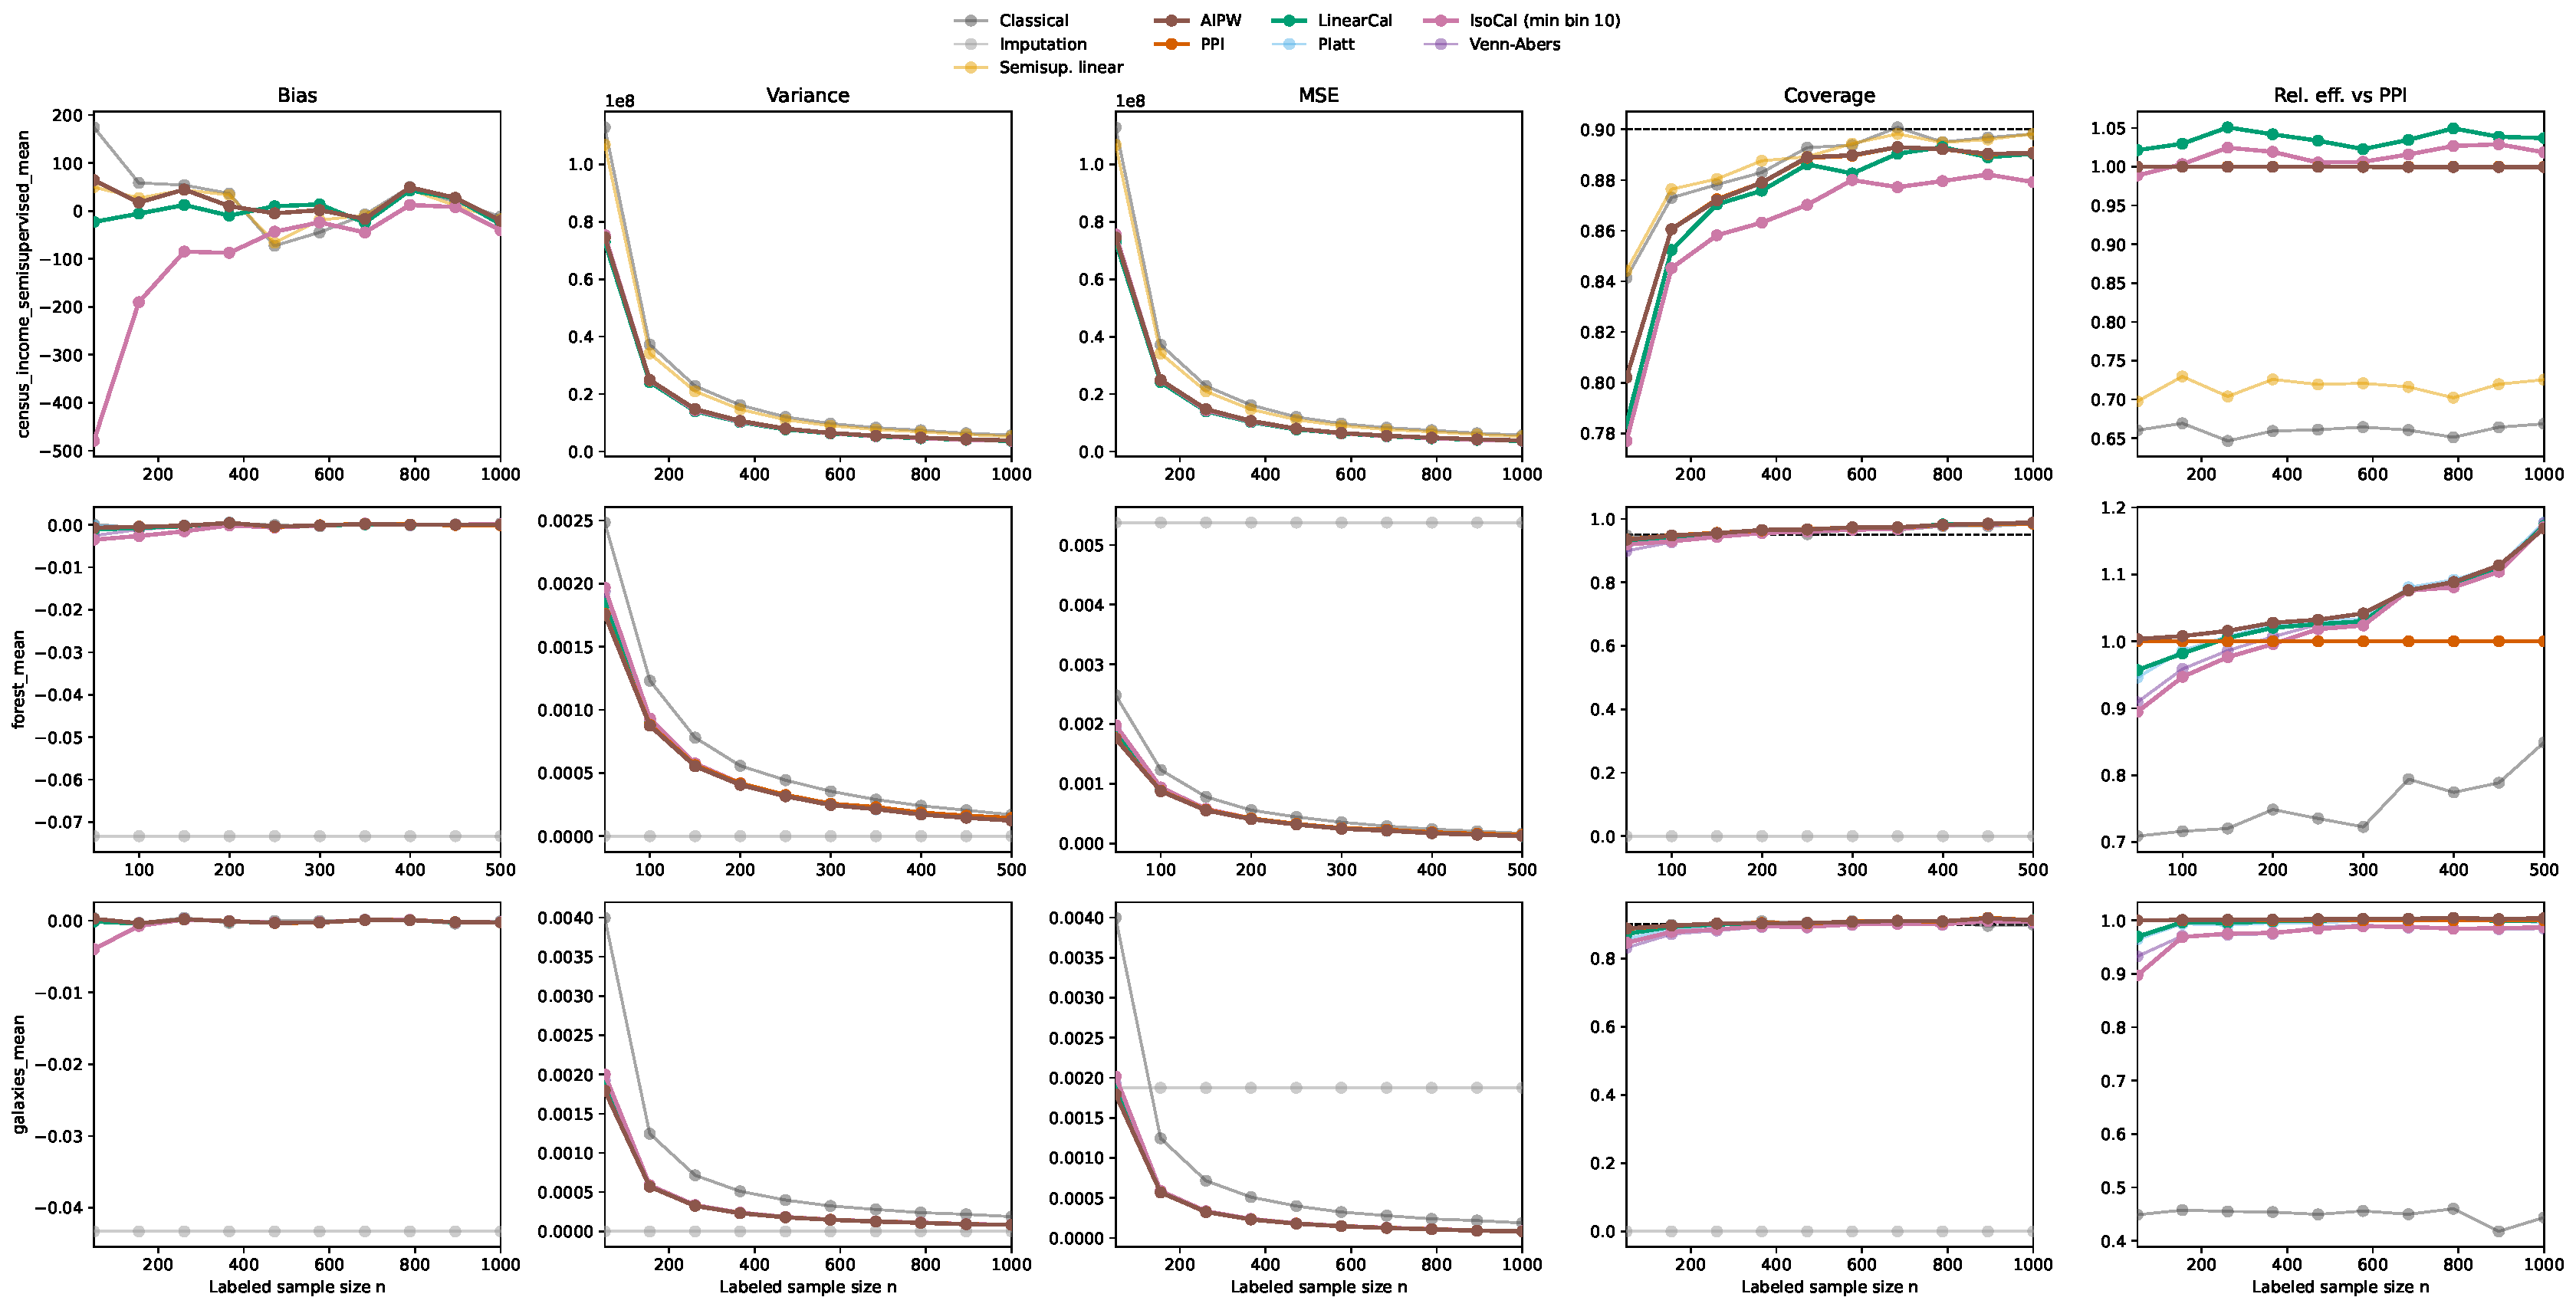
\includegraphics[width=\textwidth]{paper_assets/fig_paper_metric_grid.pdf}
\caption{Full diagnostic grid for the reproduced PPI benchmarks, showing bias, empirical variance, MSE, coverage, and relative efficiency versus PPI across labeled-sample-size regimes. The dashed horizontal line in the coverage panels marks the nominal target coverage \(1-\alpha\), and the dashed horizontal line in the relative-efficiency panels marks parity with vanilla PPI. Platt scaling and Venn--Abers appear only on the binary-outcome datasets where they are well defined.}
\label{fig:ppi-benchmarks-full}
\end{figure}

\bibliographystyle{plainnat}
\bibliography{references}

\end{document}
